%
%===============>>  ГРУППА 11-1 МОДУЛЬ 6  <<=============
%
\setmodule{6}

%BEGIN_FOLD % ====>>_____ Занятие 1 _____<<====
\begin{class}[number=1]
	\begin{listofex}
		\item Площадь грани прямоугольного параллелепипеда равна \( 15 \). Ребро, перпендикулярное этой грани, равно \(3\). Найдите объем параллелепипеда.
		\item Три ребра прямоугольного параллелепипеда, выходящие из одной вершины, равны \(4, 6, 9\). Найдите ребро равновеликого ему куба.
		\item Два ребра прямоугольного параллелепипеда, выходящие из одной вершины, равны \(3\) и \(4\). Площадь поверхности этого параллелепипеда равна \(94\). Найдите третье ребро, выходящее из той же вершины.
		\item Объем прямоугольного параллелепипеда равен \(24\). Одно из его ребер равно \(3\). Найдите площадь грани параллелепипеда, перпендикулярной этому ребру.
		\item Прямоугольный параллелепипед описан около сферы радиуса \(1\). Найдите его площадь поверхности.
		\item Диагональ куба равна \( 2\sqrt{3} \). Найдите объем куба и площадь его поверхности.
		\item Объем первого куба в \( 8 \) раз больше объема второго куба. Во сколько раз площадь поверхности первого куба больше площади поверхности второго куба?
		\item Найдите площадь боковой поверхности правильной шестиугольной призмы, сторона основания которой равна \( 5 \), а высота  --- \( 10 \).
		\item Дан куб \( ABCDA_1B_1C_1D_1 \). Площадь четырехугольника \( ABC_1D_1 \) равна \( 4\sqrt{2} \). Найдите площадь поверхности куба.
		\item 
		\begin{minipage}[t]{\bodywidth}
			В правильной треугольной пирамиде \(SABC\) с вершиной \(S\) биссектрисы треугольника \(ABC\) пересекаются в точке \(O\). Площадь треугольника \(ABC\) равна \(2\); объем пирамиды равен \(6\). Найдите длину отрезка \(OS\).
		\end{minipage}
		\hspace{0.02\linewidth}
		\begin{minipage}[t]{\picwidth}
			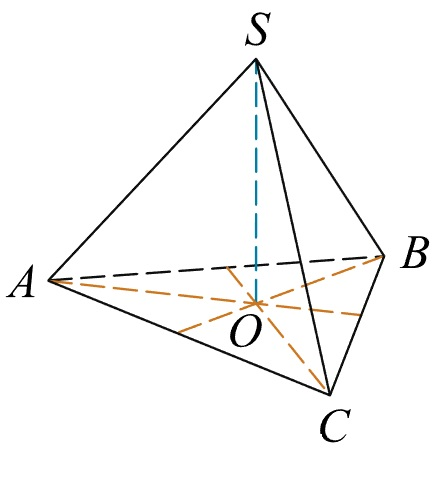
\includegraphics[align=t, width=\linewidth]{\picpath/G111M6L1-1}
		\end{minipage}
		\item В правильной четырехугольной пирамиде \(SABCD\) точка \(O\) --- центр основания, \(S\) --- вершина, \(SO=15, BD=16\). Найдите боковое ребро \(SA\).
		
		\item 
		\begin{minipage}[t]{\bodywidth}
			В правильной треугольной пирамиде \(SABC\) точка \(M\) --- середина ребра \(AB\), \(S\) --- вершина. Известно, что \(BC = 3\), а площадь боковой поверхности пирамиды равна \(45\). Найдите длину отрезка \(SM\).
		\end{minipage}
		\hspace{0.02\linewidth}
		\begin{minipage}[t]{\picwidth}
			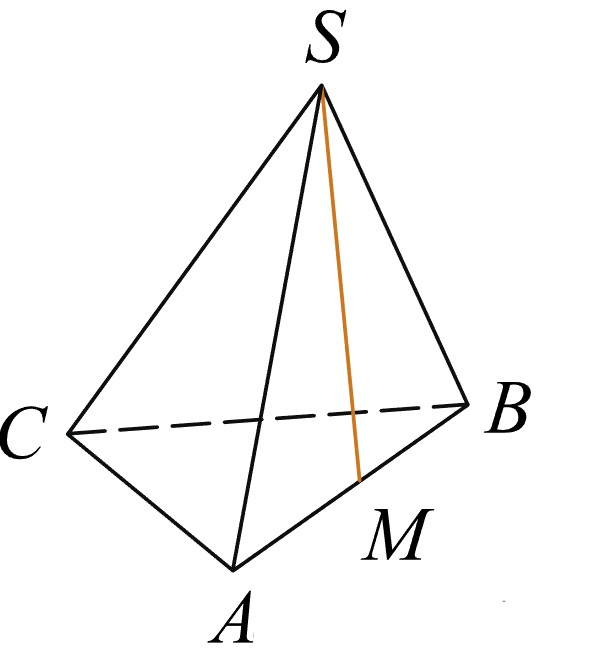
\includegraphics[align=t, width=\linewidth]{\picpath/G111M6L1-2}
		\end{minipage}
		\item Объем параллелепипеда \(ABCDA_1B_1C_1D_1\) равен \(9\). Найдите объем треугольной пирамиды \(ABCA_1\).
		\item Во сколько раз увеличится объем правильного тетраэдра, если все его ребра увеличить в два раза?
		\item В треугольнике \(ABC\) \(AB = 10, AC = BC\), высота \(AH = 8\). Найдите \(\cos{BAC}\).
		\item В треугольнике со сторонами \(9\) и \(6\) проведены высоты к этим сторонам. Высота, проведённая к первой из этих сторон, равна \(4\). Чему равна высота, проведённая ко второй стороне?
		\item Площадь параллелограмма \(ABCD\) равна \(24\). Точка \(M\) --- середина стороны \(BC\). Найдите площадь трапеции \(AMCD\).
	\end{listofex}
\end{class}
%END_FOLD

%BEGIN_FOLD % ====>>_____ Занятие 2 _____<<====
\begin{class}[number=2]
	\begin{listofex}
		\item 
		\begin{minipage}[t]{\bodywidth}
			На рисунке изображен многогранник, все двугранные углы многогранника прямые. Найдите квадрат расстояния между вершинами \(B_2\) и \(D_3\) .
		\end{minipage}
		\hspace{0.02\linewidth}
		\begin{minipage}[t]{\picwidth}
			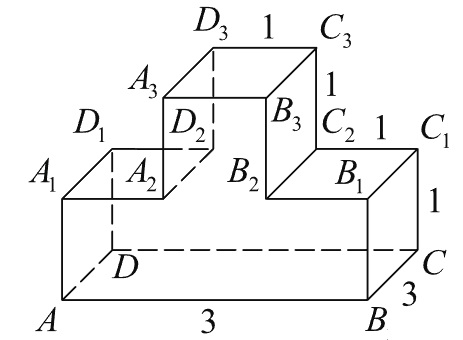
\includegraphics[align=t, width=\linewidth]{\picpath/G101M5L6-2}
		\end{minipage}
		\item С помощью этого же рисунка найдите:
		\begin{tasks}(1)
			\task расстояние между вершинами \(B\) и \(D_2\),
			\task тангенс угла \(C_2C_3B_2\).
		\end{tasks}
		\item 
		\begin{minipage}[t]{\bodywidth}
			На рисунке изображен многогранник, все двугранные углы многогранника прямые. Найдите его объём и площадь поверхности.
		\end{minipage}
		\hspace{0.02\linewidth}
		\begin{minipage}[t]{\picwidth}
			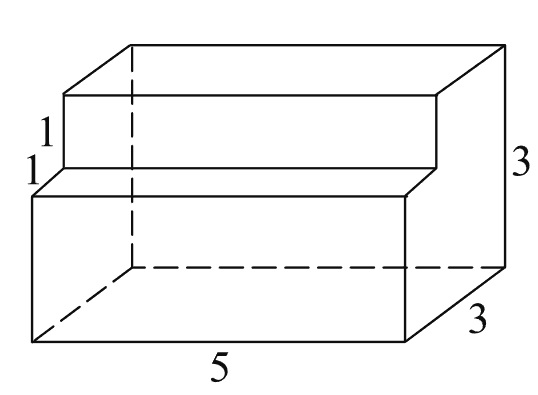
\includegraphics[align=t, width=\linewidth]{\picpath/G101M5L7-2}
		\end{minipage}

		%\item  В ДЗ!!!!!!!!!!!!!!!!!!!!!!!!!!!!!!!!!!!!!!!!!!!!!!!!!
		%\begin{minipage}[t]{\bodywidth}
		%	На рисунке изображен многогранник, все двугранные углы многогранника прямые. Найдите его объём и площадь поверхности.
		%\end{minipage}
		%\hspace{0.02\linewidth}
		%\begin{minipage}[t]{\picwidth}
		%	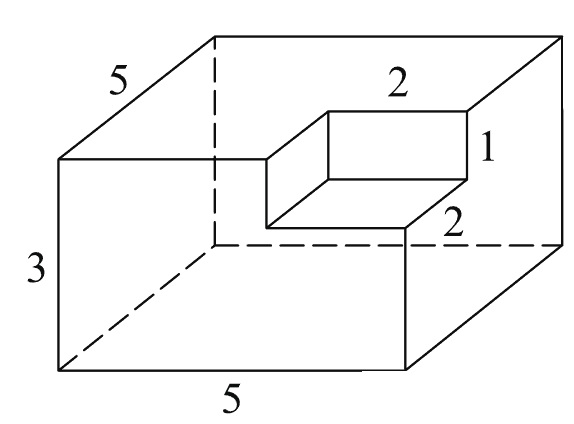
\includegraphics[align=t, width=\linewidth]{\picpath/G101M5L7-3}
		%\end{minipage}
		\item 
		\begin{minipage}[t]{\bodywidth}
			На рисунке изображен многогранник, все двугранные углы многогранника прямые. Найдите его объём и площадь поверхности.
		\end{minipage}
		\hspace{0.02\linewidth}
		\begin{minipage}[t]{\picwidth}
			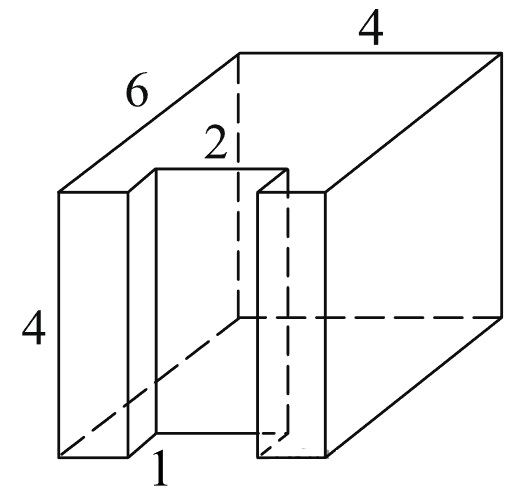
\includegraphics[align=t, width=\linewidth]{\picpath/G102M5L7-2}
		\end{minipage}
		%\item В ДЗ!!!!!!!!!!!!!!!!!!!!!!!!!!!!!!!!!!!!!!!!!!!!!!!!!УУУ
		%\begin{minipage}[t]{\bodywidth}
		%	На рисунке изображен многогранник, все двугранные углы многогранника прямые. Найдите его объём и площадь поверхности.
		%\end{minipage}
		%\hspace{0.02\linewidth}
		%\begin{minipage}[t]{\picwidth}
		%	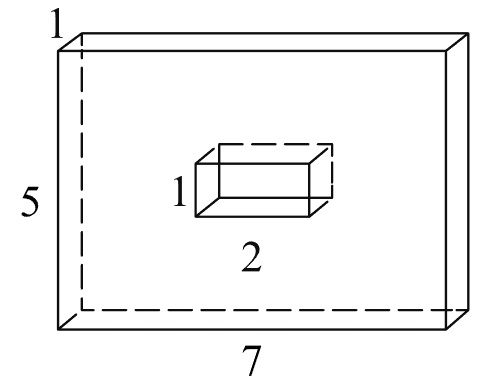
\includegraphics[align=t, width=\linewidth]{\picpath/G102M5L7-3}
		%\end{minipage}
		\item 
		\begin{minipage}[t]{\bodywidth}
			На рисунке изображён многогранник, все двугранные углы многогранника прямые. Найдите расстояние между вершинами \(A\) и \(C_2\) .
		\end{minipage}
		\hspace{0.02\linewidth}
		\begin{minipage}[t]{\picwidth}
			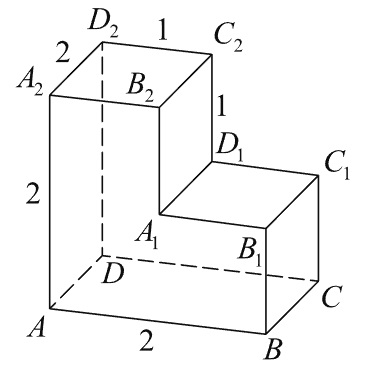
\includegraphics[align=t, width=\linewidth]{\picpath/G101M5L6-1}
		\end{minipage}
		%\item С помощью этого же рисунка найдите расстояние между вершинами:
		%\begin{tasks}(3)
			%\task \(D\) и \(C_2\),
			%\task \(B_1\) и \(D_2\),
			%\task \(D_2\) и \(A_1\).
		%\end{tasks}
		%\item С помощью этого же рисунка найдите:
		%\begin{tasks}(2)
		%	\task угол \( CAD_2 \),
		%	\task угол \( ABD \),
		%	\task тангенс угла \( B_2A_2C_2 \).
		%\end{tasks}
		\item В цилиндрический сосуд налили \(2000\) см\(^3\) воды. Уровень воды при этом достигает высоты \(12\) см. В жидкость полностью погрузили деталь. При этом уровень жидкости в сосуде поднялся на \(9\) см. Чему равен объем детали? Ответ выразите в см\(^3\).
		\item В цилиндрическом сосуде уровень жидкости достигает \(16\) см. На какой высоте будет находиться уровень жидкости, если ее перелить во второй сосуд, диаметр которого в \(2\) раза больше первого? Ответ дайте в сантиметрах.
		\item Объем первого цилиндра равен \(12\) м\(^3\). У второго цилиндра высота в три раза больше, а радиус основания --- в два раза меньше, чем у первого. Найдите объем второго цилиндра. Ответ дайте в кубических метрах.
		\item Объем конуса равен \(16\). Через середину высоты параллельно основанию конуса проведено сечение, которое является основанием меньшего конуса с той же вершиной. Найдите объем меньшего конуса.
		\item Во сколько раз уменьшится объем конуса, если его высота уменьшится в \(3\) раза, а радиус основания останется прежним?
		%\item Во сколько раз увеличится объем конуса, если радиус его основания увеличится в 1,5 раза, а высота останется прежней?
		\item Диаметр основания конуса равен \(6\), а угол при вершине осевого сечения равен \(90\pi \). Вычислите объем конуса, деленный на \( \pi \).
		\item Через среднюю линию основания треугольной призмы, объем которой равен \(32\), проведена плоскость, параллельная боковому ребру. Найдите объем отсеченной треугольной призмы.
		\item 
		\begin{minipage}[t]{\bodywidth}
			Объем параллелепипеда \(ABCDA_1B_1C_1D_1\) равен \(9\). Найдите объем треугольной пирамиды \(ABCA_1\).
		\end{minipage}
		\hspace{0.02\linewidth}
		\begin{minipage}[t]{\picwidth}
			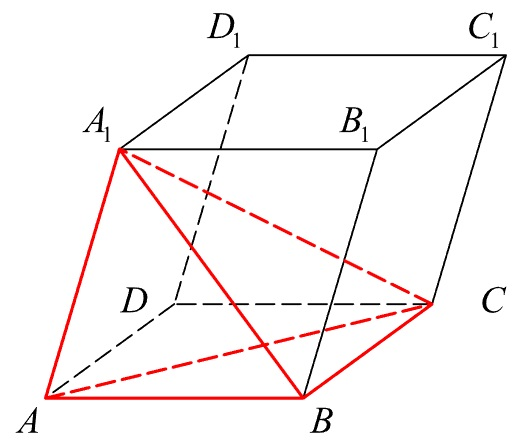
\includegraphics[align=t, width=\linewidth]{\picpath/G111M6L2-1}
		\end{minipage}
		\item Найдите корень уравнения: \( \log_5(x^2+4x-11)=5 \). Если корней несколько, в ответ запишите их сумму.
		\item Найдите корень уравнения: \( 5^{x-7}=\dfrac{1}{125} \).
	\end{listofex}
\end{class}
%END_FOLD

%BEGIN_FOLD % ====>>_ Домашняя работа 1 _<<====
\begin{homework}[number=1]
	\begin{listofex}
		\item Два ребра прямоугольного параллелепипеда, выходящие из одной вершины, равны \( 1 \), \( 2 \). Площадь поверхности параллелепипеда равна \( 16 \). Найдите его диагональ.
		\item Площадь грани прямоугольного параллелепипеда равна \( 12 \). Ребро, перпендикулярное этой грани, равно 4. Найдите объем параллелепипеда.
		\item Диагональ куба равна \( 4 \). Найдите площадь его поверхности.
		\item Ребра прямоугольного параллелепипеда равны \( 7 \), \( 12 \) и \( 5 \). Найдите объем и площадь поверхности этого параллелепипеда.
		\item В правильной треугольной пирамиде \(SABC\) медианы основания \(ABC\) пересекаются в точке \(O\). Площадь треугольника \(ABC\) равна \(9\); объем пирамиды равен \(6\). Найдите длину отрезка \(OS\).
		\item 
		\begin{minipage}[t]{\bodywidth}
			В правильной треугольной пирамиде \(SABC\) медианы основания \(ABC\) пересекаются в точке \(O\). Площадь треугольника \(ABC\) равна \(2\); объем пирамиды равен \(5\). Найдите длину отрезка \(OS\).
		\end{minipage}
		\hspace{0.02\linewidth}
		\begin{minipage}[t]{\picwidth}
		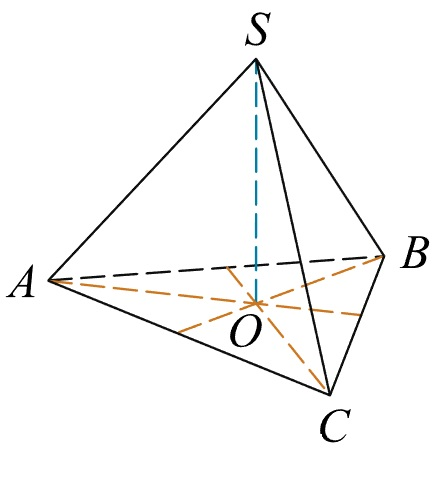
\includegraphics[align=t, width=\linewidth]{\picpath/G111M6L1-1}
		\end{minipage}
		\item 
		\begin{minipage}[t]{\bodywidth}
			В правильной четырехугольной пирамиде \(SABCD\) точка \(O\) --- центр основания, \(S\) --- вершина, \(SB=13, AC=24\). Найдите длину отрезка \(SO\).
		\end{minipage}
		\hspace{0.02\linewidth}
		\begin{minipage}[t]{\picwidth}
			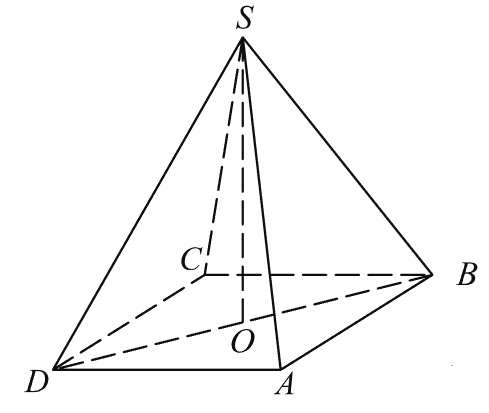
\includegraphics[align=t, width=\linewidth]{\picpath/G111M6H1-1}
		\end{minipage}
		\item В правильной четырехугольной пирамиде \(SABCD\) точка \(O\) --- центр основания, \(S\) --- вершина, \(SO=8, BD=30\). Найдите боковое ребро \(SC\).
		\item Основанием пирамиды является прямоугольник со сторонами \(3\) и \(4\). Ее объем равен \(16\). Найдите высоту этой пирамиды.
		\item Стороны основания правильной шестиугольной пирамиды равны \(10\), боковые ребра равны \(13\). Найдите площадь боковой поверхности этой пирамиды.
	\end{listofex}
\end{homework}
%END_FOLD

%BEGIN_FOLD % ====>>_____ Занятие 3 _____<<====
\begin{class}[number=3]
	\begin{definit}
		\textbf{Арксинус числа} \(a \) \((|a| \le 1) \) есть угол \( \alpha \) из промежутка \(\left[ -\dfrac{\pi}{2};\dfrac{\pi}{2} \right]\), синус которого равен \( \alpha \).%: \[ \sin{\alpha}=a \]
	\end{definit}
	\begin{definit}
		\textbf{Арккосинус числа} \(a \) \((-1\le a \le 1) \) есть угол \( \alpha \) из промежутка \([0; \pi]\), косинус которого равен \( \alpha \).%: \[ \cos{\alpha}=a \]
	\end{definit}
	\begin{definit}
		\textbf{Арктангенс числа} \(a \) есть угол \( \alpha \) из промежутка \(\left( -\dfrac{\pi}{2};\dfrac{\pi}{2} \right)\), тангенс которого равен \( \alpha \).%: \[ \tg{\alpha}=a \]
	\end{definit}
	\begin{definit}
		\textbf{Арккотангенс числа} \(a \) есть угол \( \alpha \) из промежутка \((0; \pi)\), котангенс которого равен \( \alpha \).%: \[ \cot{\alpha}=a \]
	\end{definit}
	\textbf{Формулы для отрицательного аргумента обратных тригонометрических функций}:
	\[ \arcsin{(-a)}=-\arcsin{a} \]
	\[ \arccos{(-a)}=\pi-\arccos{a} \]
	\[ \arctg{(-a)}=-\arctg{a} \]
	\[ \arcctg{(-a)}=\pi-\arcctg{a} \]
	\begin{listofex}
		\item Вычислите:
		\begin{tasks}(3)
			\task \( \arcsin{(-1)} \)
			\task \( \arcsin{\left( \dfrac{1}{2} \right)} \)
			\task \( \arcsin{\left( -\dfrac{\sqrt{3}}{2} \right)} \)
			\task \( \arccos{(-0,5)} \)
			\task \( \arcsin{\left( -\dfrac{\sqrt{2}}{2} \right)} \)
			\task \( \arcsin{\left( -\dfrac{\sqrt{3}}{2} \right)} \)
			\task \( \arctg{0} \)
			\task \( \arctg{\left( \dfrac{\sqrt{3}}{2} \right)} \)
			\task \( \arctg{\left( -\dfrac{1}{2} \right)} \)
			\task \( \arcctg{-1} \)
			\task \( \arcctg{\left( \dfrac{1}{2} \right)} \)
			\task \( \arcctg{\left( -\dfrac{2}{2} \right)} \)
		\end{tasks}
		\newpage
		\item Решите уравнения:
		\begin{tasks}(2)
			\task \( \sin x=\dfrac{1}{2} \)
			\task \( \cos x=-\dfrac{\sqrt{3}}{2} \)
			\task \( \sin x = -\dfrac{\sqrt{2}}{2} \)
			\task \( \tg x = \dfrac{-\sqrt{3}}{3} \)
			\task \( \ctg x = -1 \)
			\task \( \cos x = \dfrac{\sqrt{2}}{2} \)
		\end{tasks}
		\item Решить уравнения:
		\begin{tasks}(2)
			\task \( \cos\left( 2x+\dfrac{\pi}{4} \right)=\dfrac{\sqrt{2}}{2} \)
			\task \( \sin \left( 2x-\dfrac{3\pi}{2} \right) = -1 \)
			\task \( \cos \left( \dfrac{\pi}{4}-x \right)=\dfrac{\sqrt{3}}{2} \)
			\task \( \ctg\left( 2x-\dfrac{3\pi}{4} \right)=-1 \)
		\end{tasks}
		\item Решить уравнение \( \cos\dfrac{\pi(x-7)}{3}=\dfrac{1}{2} \). В ответ запишите наибольший отрицательный корень.
		\item Решить уравнение \( \tg\dfrac{\pi x}{4}=\dfrac{1}{2} \). В ответ запишите наибольший отрицательный корень.
		\item Решить уравнение \( \cos\dfrac{\pi(x-4)}{2}=\dfrac{3}{2} \). В ответ запишите наибольший отрицательный корень.
		\item Решить уравнение \( \sin\dfrac{2\pi x}{3}=\dfrac{1}{2} \). В ответ запишите наибольший отрицательный корень.
		\item Решить уравнение \( \cos\dfrac{\pi(3x+6)}{3}=\dfrac{\sqrt{2}}{2} \). В ответ запишите наименьший положительный корень.
		%\item Заказ на \(110\) деталей первый рабочий выполняет на \(1\) час быстрее, чем второй. Сколько деталей за час изготавливает второй рабочий, если известно, что первый за час изготавливает на \(1\) деталь больше?
		\item На изготовление \(475\) деталей первый рабочий тратит на \(6\) часов меньше, чем второй рабочий на изготовление \(550\) таких же деталей. Известно, что первый рабочий за час делает на \(3\) детали больше, чем второй. Сколько деталей в час делает первый рабочий?
		%\item Двое рабочих, работая вместе, могут выполнить работу за \(12\) дней. За сколько дней, работая отдельно, выполнит эту работу первый рабочий, если он за два дня выполняет такую же часть работы, какую второй  --- за три дня?
		\item Поезд, двигаясь равномерно со скоростью \(80\) км/ч, проезжает мимо столба, за \(36\) секунд. Найдите длину поезда в метрах.
		%\item Поезд, двигаясь равномерно со скоростью \(63\) км/ч, проезжает мимо пешехода, идущего в том же направлении параллельно путям со скоростью \(3\) км/ч, за \(39\) секунд. Найдите длину поезда в метрах.
		\item Сколько времени будет проходить поезд длиной \(500\) м через тоннель, длина которого \(500\) м, если скорость поезда \(60\) км/ч?
		%\item Два велосипедиста одновременно отправились в \(88\)-километровый пробег. Первый ехал со скоростью, на \(3\) км/ч большей, чем скорость второго, и прибыл к финишу на \(3\) часа раньше второго. Найти скорость велосипедиста, пришедшего к финишу вторым. Ответ дайте в км/ч.
		%\item По двум параллельным железнодорожным путям друг навстречу другу следуют скорый и пассажирский поезда, скорости которых равны соответственно \(60\) км/ч и \(30\) км/ч. Длина пассажирского поезда равна \(400\) метрам. Найдите длину скорого поезда, если время, за которое он прошел мимо пассажирского поезда, равно 38 секундам. Ответ дайте в метрах.
	\end{listofex}
\end{class}
%END_FOLD

%BEGIN_FOLD % ====>>_____ Занятие 4 _____<<====
\begin{class}[number=4]
	\title{Самостоятельное прорешивание (30 минут)}
	\begin{listofex}
		\item Боковая сторона равнобедренного треугольника равна \( 7 \), угол при вершине, противолежащей основанию, равен \( 120\degree \). Найдите диаметр описанной окружности этого треугольника.
		\item Объем параллелепипеда \( ABCDA_1B_1C_1D_1 \) равен \( 9 \). Найдите объем треугольной пирамиды \( ABCA_1 \).
		\item На изготовление \( 99 \) деталей первый рабочий тратит на \( 2 \) часа меньше, чем второй рабочий на изготовление \( 110 \) таких же деталей. Известно, что первый рабочий за час делает на \( 1 \) деталь больше, чем второй. Сколько деталей в час делает второй рабочий?
		\item Фабрика выпускает сумки. В среднем на \( 190 \) качественных сумок приходится восемь сумок со скрытыми дефектами. Найдите вероятность того, что купленная сумка окажется качественной. Результат округлите до сотых.
		\item Вероятность того, что батарейка бракованная, равна \( 0,06 \). Покупатель в магазине выбирает случайную упаковку, в которой две таких батарейки. Найдите вероятность того, что обе батарейки окажутся исправными.
		\item На рисунке изображён график функции вида \( f(x)=\dfrac{x^2}{a}+bx+c \),  где числа \( a \), \( b \) и \( c \) --- целые. Найдите значение \( f(4) \).
		\begin{center}
			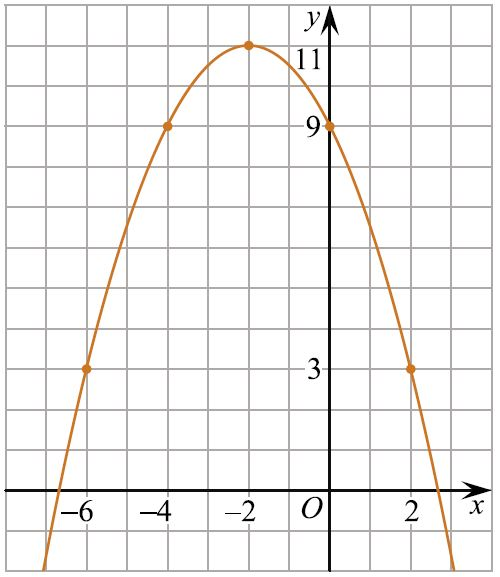
\includegraphics[align=t, width=0.4\linewidth]{\picpath/G112M3C2-4}
		\end{center}
	\end{listofex}
	\newpage
	\title{Основная часть занятия}
	\begin{listofex}
		\item Решите уравнения:
		\begin{tasks}(2)
			\task \( \sin x=-\dfrac{1}{2} \)
			\task \( \cos x=-\dfrac{\sqrt{3}}{2} \)
			\task \( \sin x = -\dfrac{\sqrt{3}}{2} \)
			\task \( \tg x = \dfrac{\sqrt{3}}{3} \)
			\task \( \ctg^2 x = 1 \)
			\task \( \cos^2 x = \dfrac{\sqrt{2}}{2} \)
		\end{tasks}
		\item Решить уравнение: \( \tg\dfrac{\pi x}{4}=\dfrac{1}{2} \). В ответ запишите наибольший отрицательный корень.
		\item Решить уравнение: \( \cos\dfrac{\pi(x-4)}{2}=\dfrac{3}{2} \). В ответ запишите наибольший отрицательный корень.
		\item Решить уравнение: \( \sin\dfrac{2\pi x}{3}=\dfrac{1}{2} \). В ответ запишите наибольший отрицательный корень.
		\item Решить уравнение: \( \cos\dfrac{\pi(3x+6)}{3}=\dfrac{\sqrt{2}}{2} \). В ответ запишите наименьший положительный корень.
		%\item Решить уравнение \( \cos\dfrac{\pi(x-7)}{3}=\dfrac{1}{2} \). В ответ запишите наибольший отрицательный корень.
		%\item Решить уравнение \( \tg\dfrac{\pi x}{4}=\dfrac{1}{2} \). В ответ запишите наибольший отрицательный корень.
		%\item Решить уравнение \( \cos\dfrac{\pi(x-4)}{2}=\dfrac{3}{2} \). В ответ запишите наибольший отрицательный корень.
		%\item Решить уравнение \( \sin\dfrac{2\pi x}{3}=\dfrac{1}{2} \). В ответ запишите наибольший отрицательный корень.
		%\item Решить уравнение \( \cos\dfrac{\pi(3x+6)}{3}=\dfrac{\sqrt{2}}{2} \). В ответ запишите наименьший положительный корень.
		\item Первая труба пропускает на \(1\) литр воды в минуту меньше, чем вторая. Сколько литров воды в минуту пропускает вторая труба, если резервуар объемом \(110\) литров она заполняет на \(1\) минуту быстрее, чем первая труба?
		\item Первая труба пропускает на \(1\) литр воды в минуту меньше, чем вторая. Сколько литров воды в минуту пропускает первая труба, если резервуар объемом \(110\) литров она заполняет на \(2\) минуты дольше, чем вторая труба заполняет резервуар объемом \(99\) литров?
		\item Из двух городов, расстояние между которыми равно \(560\) км, навстречу друг другу одновременно выехали два автомобиля. Через сколько часов автомобили встретятся, если их скорости равны \(65\) км/ч и \(75\) км/ч?
	\end{listofex}
\end{class}
%END_FOLD

%BEGIN_FOLD % ====>>_ Домашняя работа 2 _<<====
\begin{homework}[number=2]
	\begin{listofex}
		\item Решить уравнение \( \sin\dfrac{\pi(4x-3)}{4}=1 \). В ответ запишите наибольший отрицательный корень.
		\item Решить уравнение \( \sin\dfrac{\pi(8x+3)}{6}=0,5 \). В ответ запишите наименьший положительный корень.
		\item Решить уравнение \( \cos\dfrac{\pi(x+1)}{4}=\dfrac{\sqrt{2}}{2} \). В ответ запишите наибольший отрицательный корень.
		\item Решить уравнение \( \cos\dfrac{\pi(4x+1)}{6}=\dfrac{\sqrt{3}}{2} \). В ответ запишите наибольший отрицательный корень.
		\item Решить уравнение \( \tg\dfrac{\pi(x-3)}{6}=\dfrac{1}{\sqrt{3}} \). В ответ запишите наибольший отрицательный корень.
		\item Решить уравнение \( \tg\dfrac{\pi(4x-5)}{4}=-1 \). В ответ запишите наименьший положительный корень.
		\item Заказ на \(156\) деталей первый рабочий выполняет на \(1\) час быстрее, чем второй. Сколько деталей за час изготавливает первый рабочий, если известно, что он за час изготавливает на \(1\) деталь больше второго?
		%\item На изготовление \(99\) деталей первый рабочий тратит на \(2\) часа меньше, чем второй рабочий на изготовление \(110\) таких же деталей. Известно, что первый рабочий за час делает на \(1\) деталь больше, чем второй. Сколько деталей в час делает второй рабочий?
		\item Первая труба пропускает на \(1\) литр воды в минуту меньше, чем вторая. Сколько литров воды в минуту пропускает первая труба, если резервуар объемом \(110\) литров она заполняет на \(1\) минуту дольше, чем вторая труба?
		\item По двум параллельным железнодорожным путям в одном направлении следуют пассажирский и товарный поезда, скорости которых равны соответственно \(40\) км/ч и \(60\) км/ч. Длина товарного поезда равна \(700\) м. Найдите длину пассажирского поезда, если время, за которое он прошел мимо товарного поезда, равна \(3\) мин. Ответ дайте в метрах.
		%\item По морю параллельными курсами в одном направлении следуют два сухогруза: первый длиной \(140\) метров, второй --- длиной \(60\) метров. Сначала второй сухогруз отстает от первого, и в некоторый момент времени расстояние от кормы первого сухогруза до носа второго составляет \(800\) метров. Через \(15\) минут после этого уже первый сухогруз отстает от второго так, что расстояние от кормы второго сухогруза до носа первого равно \(1000\) метрам. На сколько километров в час скорость первого сухогруза меньше скорости второго?
	\end{listofex}
\end{homework}
%END_FOLD

%BEGIN_FOLD % ====>>_____ Занятие 5 _____<<====
\begin{class}[number=5]
	\begin{listofex}
		\item Решите уравнения:
		\begin{tasks}(2)
			\task \( 6\cos^2{x}+\cos{x}-1=0 \)
			\task \( 2\cos^2{3x}-5\cos{3x}-3=0 \)
			\task \( 2\cos^2{\dfrac{x}{3}}+3\cos{\dfrac{x}{3}}-2=0 \)
			%\task \( 2\sin^2x+3\cos{x}=0 \)
			\task \( 8\sin^2{2x}+\cos{2x}+1=0 \)
			%\task \( 5\cos^2{2x}+6\sin{2x}-6=0 \) V DZ
			%\task \( 4\sin{3x}+\cos^2{3x}=4 \) V DZ
			%\task \( 3\tg^2{x}+2\tg{x}-1=0 \) V DZ
			\task \( \ctg^2{2x}-6\ctg{2x}+5=0 \)
		\end{tasks}
		\item Решите уравнения:
		\begin{tasks}(1)
			\task \( \sin{2x}+2\sin{(-x)}+\cos{(-x)}-1=0 \)
			\task \( \cos{2x}+\sqrt{2}\cos{\left( \dfrac{\pi}{2}-x \right)}-1=0 \)
			\task \( 7\sin{ \left( \dfrac{\pi}{2}+x \right) +4\sqrt{3}\sin{x} \cos{x} = 4 \cos^3{x}  } \)
			\task \( \sin{(\pi-x)}- \cos{\left( \dfrac{\pi}{2}+x \right) = -1 }  \)
		\end{tasks}
	\end{listofex}
\end{class}
%END_FOLD
	
%BEGIN_FOLD % ====>>_____ Занятие 6 _____<<====
\begin{class}[number=6]
	\begin{listofex}
		\item Решите уравнения:
		\begin{tasks}(1)
			\task \( \tg{\left( 2x-\dfrac{\pi}{3} \right)}=\dfrac{\sqrt{3}}{3} \)
			\task \( \ctg{\left( \dfrac{x}{3}-\dfrac{\pi}{3} \right)} = \dfrac{\sqrt{3}}{3} \)
			\task \( 5 \sin^2{x}-7\sin{x} \cos{x} + 4 \cos^2{x}=1 \)
			\task \( 3\cos^2{x}-\sin{2x}=0,5 \)
			\task \( \sin{2x}+5\sin^2{x}=1,5 \)
			\task \( 2\cos{2x}-\cos^3{x}=2-16\cos^2{x} \)
		\end{tasks}
		\item Решите уравнения:
		\begin{tasks}(1)
			\task \( \cos{2x}=1-\cos{\left( \dfrac{\pi}{2}-x \right) } \)
			\task \( 4\sin^3{x}=3\cos{\left( x-\dfrac{\pi}{2} \right) } \)
			\task \( -\sqrt{2}\sin{\left( -\dfrac{5\pi}{2}+x \right) \cdot \sin{x} = \cos{x} } \)
			\task \( 2\cos{x}-\sqrt{3}\sin^2{x}=2\cos^3{x} \)
		\end{tasks}
	\end{listofex}
\end{class}
%END_FOLD
	
%BEGIN_FOLD % ====>>_ Домашняя работа 3 _<<====
\begin{homework}[number=3]
	\begin{listofex}
		\item Решите уравнения:
		\begin{tasks}(1)
			\task \( 2\sin^2x+3\cos{x}=0 \)
			\task \( 5\cos^2{2x}+6\sin{2x}-6=0 \)
			\task \( 4\sin{3x}+\cos^2{3x}=4 \)
			\task \( 3\tg^2{x}+2\tg{x}-1=0 \)
			%\task \( 2x\cos{x}-8\cos{x}+x-4=0 \)
			%\task \( 2\sin{(\pi+x)}\cdot \sin{0,5\pi+x}=\sin{x} \)
		\end{tasks}
		\item Решите уравнения:
		\begin{tasks}(1)
			\task \( 2\sin{2x}=4\cos{x}-\sin{x}+1 \)
			\task \( \sin{2x}+\sqrt{2}\sin{x}=2\cos{x}+\sqrt{2} \)
			\task \( \cos^2{x}-\dfrac{1}{2} \cdot \sin{2x} + \cos{x} = \sin{x} \)
		\end{tasks}
		\item Решите уравнения:
		\begin{tasks}
			\task \( \cos{\left( \dfrac{\pi}{2}+2x \right)} = \sqrt{2} \sin{x} \)
			\task \( 2\sin{ \left( \dfrac{7\pi}{2}-x \right)} \sin{x}=\cos{x} \)
		\end{tasks}
	\end{listofex}
\end{homework}
%END_FOLD

%BEGIN_FOLD % ====>>_____ Занятие 7 _____<<====
\begin{class}[number=7]
	\begin{listofex}
		\item
		\begin{tasks}
			\task Решите уравнение: \( 3\sqrt{3} \cos{\left( \dfrac{3\pi}{2} + x \right)} -3=2\sin^2{x}  \),
			\task Найдите корни на промежутке: \( [2\pi;3\pi] \).
		\end{tasks}
		\item
		\begin{tasks}
			\task Решите уравнение: \( 3\sqrt{2}\sin{\left( \dfrac{\pi}{2} + x \right)} -2 = 2\cos^2{x} \),
			\task Найдите корни на промежутке: \( \left[ \dfrac{3\pi}{2}; \dfrac{5\pi}{2} \right] \).
		\end{tasks}
		\item
		\begin{tasks}
			\task Решите уравнение: \( \sin^2{x}+\sin^2{\dfrac{\pi}{6}}= \cos^2{2x} + \cos^2{\dfrac{\pi}{3}} \),
			\task Найдите корни на промежутке: \( \left[ \dfrac{7\pi}{2}; \dfrac{9\pi}{2} \right) \).
		\end{tasks}
		\item
		\begin{tasks}
			\task Решите уравнение: \( \cos^2{x}+\cos^2{\dfrac{\pi}{6}} = \cos^2{2x} + \sin^2{\dfrac{\pi}{3}} \),
			\task Найдите корни на промежутке: \( \left( \dfrac{7\pi}{2}; \dfrac{9\pi}{2} \right] \).
		\end{tasks}
		\item
		\begin{tasks}
			\task Решите уравнение: \( 8 \sin{x}+4\cos^2{x}=7 \),
			\task Найдите корни на промежутке: \( \left[ -\dfrac{3\pi}{2}; -\dfrac{\pi}{2} \right]  \).
		\end{tasks}
		\item
		\begin{tasks}
			\task Решите уравнение: \( 2 \cos^2{x} + 19 \sin{x}+8=0 \),
			\task Найдите корни на промежутке: \( \left[ -\pi; \dfrac{\pi}{2} \right]  \).
		\end{tasks}
	\end{listofex}
\end{class}
%END_FOLD

%BEGIN_FOLD % ====>>_ Проверочная работа _<<====
\begin{class}[number=8]
	\begin{listofex}
		\item % СБОРНИК КАЗАРОВА, УРАВНЕНИЕ 7 стр 1 И ПОТОМ номера 1-2 всех страниц
		\begin{tasks}
			\task Решите уравнение: \( \cos{2x}+3\sin{x}-2=0 \), %7
			\task Найдите корни на промежутке: \( [-3\pi;-\pi] \).
		\end{tasks}
		\item %11
		\begin{tasks}
			\task Решите уравнение: \( \sin{x} \cdot (2\sin{x}-1) + \sqrt{3} \sin{x} + \sin{\dfrac{4\pi}{3}}=0 \), 
			\task Найдите корни на промежутке: \( \left[ -\dfrac{\pi}{2};\pi \right) \).
		\end{tasks}
		\item % 12
		\begin{tasks}
			\task Решите уравнение: \( 2\cos{x} \cdot \left( \cos{x}+\cos{\dfrac{5\pi}{4}} \right) + \cos{x} + \cos{\dfrac{3\pi}{4}}=0  \),
			\task Найдите корни на промежутке: \( \left[ \pi; \dfrac{5\pi}{2} \right) \).
		\end{tasks}
		\item %21
		\begin{tasks}
			\task Решите уравнение: \( 2(\cos{x}-1)\sin{2x}=3 \cos{ \left( \dfrac{3\pi}{2}+x \right) } \),
			\task Найдите корни на промежутке: \( \left[ \dfrac{3\pi}{2}; 3\pi \right] \).
		\end{tasks}
		\item %22
		\begin{tasks}
			\task Решите уравнение: \( (1+2\sin{x})\sin{x}=\sin{2x}+\sin{ \left( \dfrac{\pi}{2}-x \right) } \),
			\task Найдите корни на промежутке: \( \left[ -\dfrac{3\pi}{2}; 0 \right]  \).
		\end{tasks}
		\item %31
		\begin{tasks}
			\task Решите уравнение: \( 1-2\sin^2{2x}=\sin^2{\left( \dfrac{3\pi}{2} + 4x \right) } \),
			\task Найдите корни на промежутке: \( \left[ -\dfrac{\pi}{2}; \dfrac{\pi}{2} \right] \).
		\end{tasks}
		\item % 33
		\begin{tasks}
			\task Решите уравнение: \( \sqrt{3} \cos{ \left( \dfrac{5\pi}{2}-x \right) } + \cos{2x}=1 \),
			\task Найдите корни на промежутке: \( \left[ \dfrac{5\pi}{2}; 4\pi \right] \).
		\end{tasks}
		\item %34
		\begin{tasks}
			\task Решите уравнение: \( \cos{2x} + \sqrt{3} \sin{ \left( \dfrac{3\pi}{2}+x \right)}=-1  \),
			\task Найдите корни на промежутке: \( \left[ -4 \pi ; -\dfrac{5\pi}{2} \right] \).
		\end{tasks}
	\end{listofex}
\end{class}
%END_FOLD

%BEGIN_FOLD % ====>>_ Консультация _<<====
\begin{consultation}
	\begin{listofex}
		\item 
		\begin{minipage}[t]{\bodywidth}
			На рисунке изображен многогранник, все двугранные углы многогранника прямые. Найдите площадь поверхности.
		\end{minipage}
		\hspace{0.02\linewidth}
		\begin{minipage}[t]{\picwidth}
			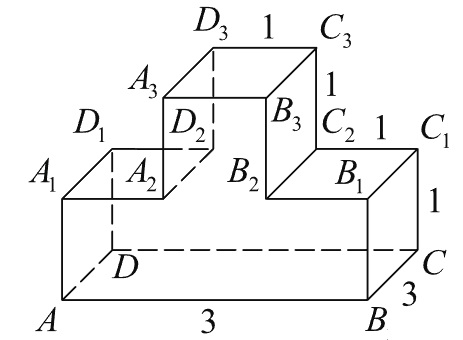
\includegraphics[align=t, width=\linewidth]{\picpath/G101M5L6-2}
		\end{minipage}
		\item 
		\begin{minipage}[t]{\bodywidth}
			На рисунке изображен многогранник, все двугранные углы многогранника прямые. Найдите его объём и площадь поверхности.
		\end{minipage}
		\hspace{0.02\linewidth}
		\begin{minipage}[t]{\picwidth}
			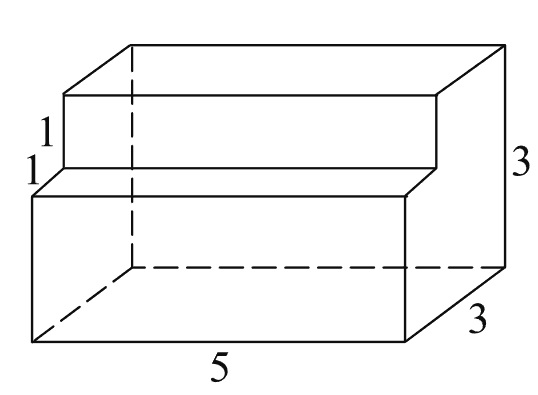
\includegraphics[align=t, width=\linewidth]{\picpath/G101M5L7-2}
		\end{minipage}
		\item 
		\begin{minipage}[t]{\bodywidth}
			На рисунке изображен многогранник, все двугранные углы многогранника прямые. Найдите его объём и площадь поверхности.
		\end{minipage}
		\hspace{0.02\linewidth}
		\begin{minipage}[t]{\picwidth}
			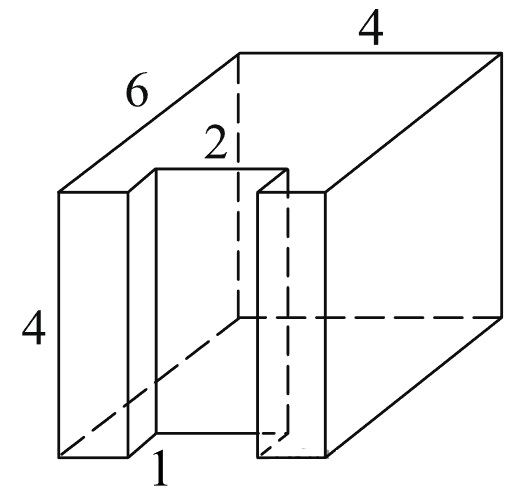
\includegraphics[align=t, width=\linewidth]{\picpath/G102M5L7-2}
		\end{minipage}
		
		\item 
		\begin{minipage}[t]{\bodywidth}
			На рисунке изображён многогранник, все двугранные углы многогранника прямые. Найдите площадь поверхности.
		\end{minipage}
		\hspace{0.02\linewidth}
		\begin{minipage}[t]{\picwidth}
			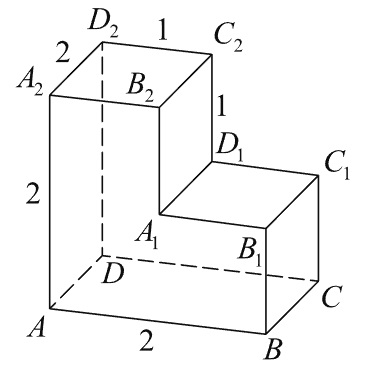
\includegraphics[align=t, width=\linewidth]{\picpath/G101M5L6-1}
		\end{minipage}
		\item 
		\begin{minipage}[t]{\bodywidth}
			На рисунке изображён многогранник, все двугранные углы многогранника прямые. Найдите площадь поверхности.
		\end{minipage}
		\hspace{0.02\linewidth}
		\begin{minipage}[t]{\picwidth}
			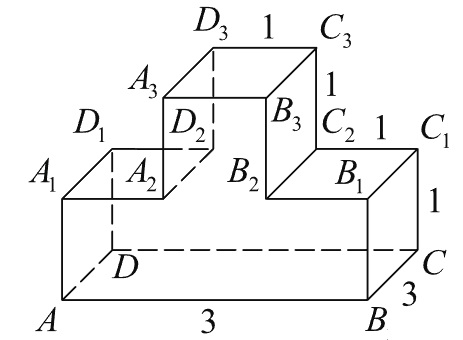
\includegraphics[align=t, width=\linewidth]{\picpath/G101M5L6-2}
		\end{minipage}
		\item Объем первого куба в \( 2 \) раза меньше объема второго куба. Во сколько раз площадь поверхности первого куба больше площади поверхности второго куба?
		\item 
		\begin{minipage}[t]{\bodywidth}
			Найдите площадь поверхности и объём пространственного креста, изображенного на рисунке и составленного из единичных кубов.
		\end{minipage}
		\hspace{0.02\linewidth}
		\begin{minipage}[t]{\picwidth}
			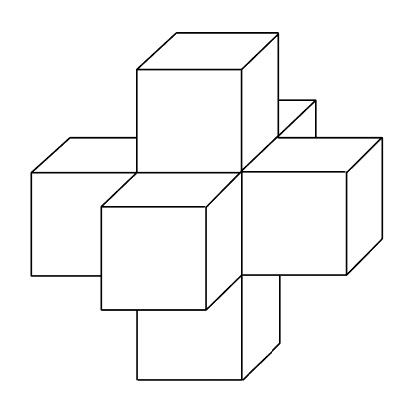
\includegraphics[align=t, width=\linewidth]{\picpath/G101M5L7-4}
		\end{minipage}
		\item 
		\begin{minipage}[t]{\bodywidth}
			На рисунке изображен многогранник, все двугранные углы многогранника прямые. Найдите его объём и площадь поверхности.
		\end{minipage}
		\hspace{0.02\linewidth}
		\begin{minipage}[t]{\picwidth}
			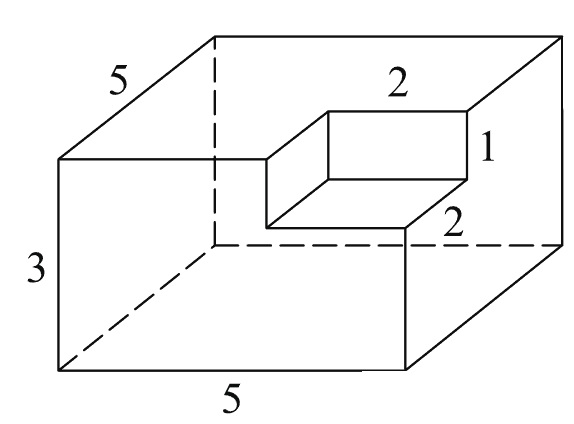
\includegraphics[align=t, width=\linewidth]{\picpath/G101M5L7-3}
		\end{minipage}
		\item
		\begin{minipage}[t]{\bodywidth}
			На рисунке изображен многогранник, все двугранные углы многогранника прямые. Найдите его объём и площадь поверхности.
		\end{minipage}
		\hspace{0.02\linewidth}
		\begin{minipage}[t]{\picwidth}
			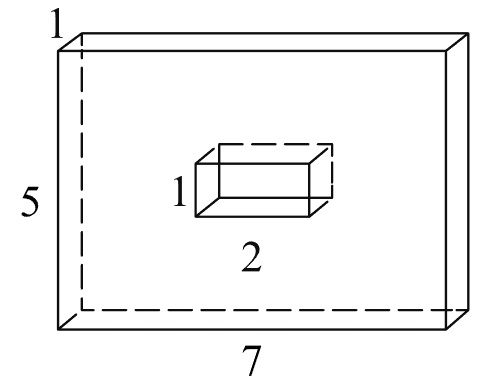
\includegraphics[align=t, width=\linewidth]{\picpath/G102M5L7-3}
		\end{minipage}
		\item
		\begin{minipage}[t]{\bodywidth}
			На рисунке изображен многогранник, все двугранные углы многогранника прямые. Найдите его объём и площадь поверхности.
		\end{minipage}
		\hspace{0.02\linewidth}
		\begin{minipage}[t]{\picwidth}
			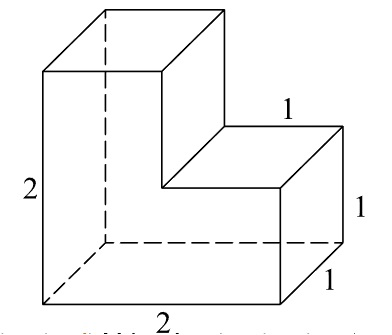
\includegraphics[align=t, width=\linewidth]{\picpath/G111M6C1-1}
		\end{minipage}
		\item Площадь грани правильного параллелепипеда равна \( 12 \). Площадь грани, перпендикулярного ей, равно \(16\). Найдите объем параллелепипеда.
	\end{listofex}
	\newpage
	\title{Домашняя работа}
	\begin{listofex}
		\item
		\begin{minipage}[t]{\bodywidth}
			На рисунке изображен многогранник, все двугранные углы многогранника прямые. Найдите его объём и площадь поверхности.
		\end{minipage}
		\hspace{0.02\linewidth}
		\begin{minipage}[t]{\picwidth}
			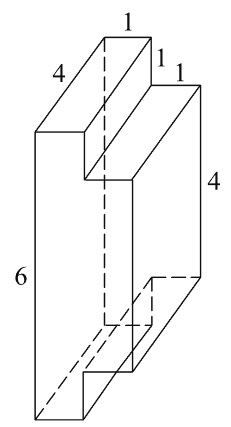
\includegraphics[align=t, width=\linewidth]{\picpath/G111M6C1-2}
		\end{minipage}
		\item
		\begin{minipage}[t]{\bodywidth}
			На рисунке изображен многогранник, все двугранные углы многогранника прямые. Найдите его объём и площадь поверхности.
		\end{minipage}
		\hspace{0.02\linewidth}
		\begin{minipage}[t]{\picwidth}
			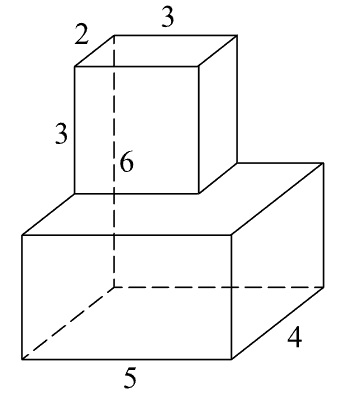
\includegraphics[align=t, width=\linewidth]{\picpath/G111M6C1-3}
		\end{minipage}
		\item
		\begin{minipage}[t]{\bodywidth}
			На рисунке изображен многогранник, все двугранные углы многогранника прямые. Найдите его объём и площадь поверхности.
		\end{minipage}
		\hspace{0.02\linewidth}
		\begin{minipage}[t]{\picwidth}
			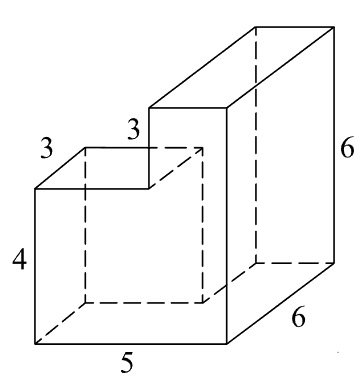
\includegraphics[align=t, width=\linewidth]{\picpath/G111M6C1-4}
		\end{minipage}
		\item
		\begin{minipage}[t]{\bodywidth}
			На рисунке изображен многогранник, все двугранные углы многогранника прямые. Найдите его объём и площадь поверхности.
		\end{minipage}
		\hspace{0.02\linewidth}
		\begin{minipage}[t]{\picwidth}
			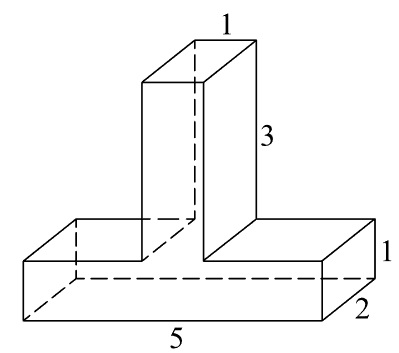
\includegraphics[align=t, width=\linewidth]{\picpath/G111M6C1-5}
		\end{minipage}
		\item
		\begin{minipage}[t]{\bodywidth}
			На рисунке изображен многогранник, все двугранные углы многогранника прямые. Найдите его объём и площадь поверхности.
		\end{minipage}
		\hspace{0.02\linewidth}
		\begin{minipage}[t]{\picwidth}
			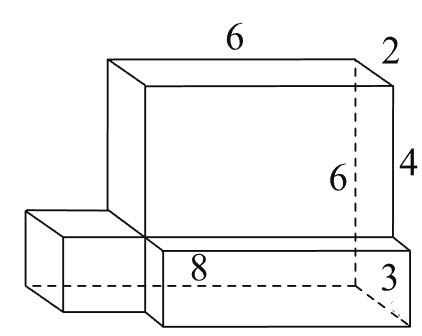
\includegraphics[align=t, width=\linewidth]{\picpath/G111M6C1-6}
		\end{minipage}
		\item Объем первого куба в \( 8 \) раза меньше объема второго куба. Во сколько раз площадь поверхности первого куба больше площади поверхности второго куба?
		\item Площадь грани правильного параллелепипеда равна \( 5\sqrt{3} \). Площадь грани, перпендикулярного ей, равно \(12\). Найдите объем и площадь поверхности параллелепипеда.
	\end{listofex}
\end{consultation}
%END_FOLD

%BEGIN_FOLD % ====>>_ Консультация _<<====
\begin{consultation}
	\begin{listofex}
		\item Решите уравнения:
		\begin{tasks}(1)
			\task \( (2x+7)^2=(2x-1)^2 \),
			\task \( \dfrac{1}{9x-7}=0,5 \),
			\task \( \sqrt{15-2x}=3 \).
		\end{tasks}
		\item Найдите значение выражения:
		\begin{tasks}(2)
			\task \( \left( \mfrac{2}{4}{7} - 1,2 \right) \cdot \mfrac{5}{5}{6} \),
			\task \( (432^2-568^2) : 1000 \),
			\task \( \dfrac{(11a)^2-11a}{11a^2-a} \).
		\end{tasks}
		\item
		\begin{minipage}[t]{\bodywidth}
			На рисунке изображён график функции вида \[ f(x)=ax-|bx+c|+d, \] где числа \(a, b, c, d\) --- целые.\\ Найдите корень уравнения \(ax+d=19\).
		\end{minipage}
		\hspace{0.02\linewidth}
		\begin{minipage}[t]{\picwidth}
			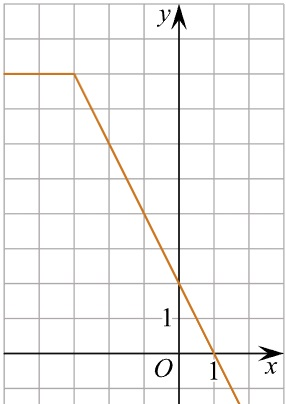
\includegraphics[align=t, width=\linewidth]{\picpath/K-L8}
		\end{minipage}
		%2
		\item
		\begin{minipage}[t]{\bodywidth}
			На рисунке изображён график функции вида \[ f(x)=ax+|bx+c|+d, \] где числа \(a, b, c, d\) --- целые.\\ Найдите корень уравнения \(bx+c=0\).
		\end{minipage}
		\hspace{0.02\linewidth}
		\begin{minipage}[t]{\picwidth}
			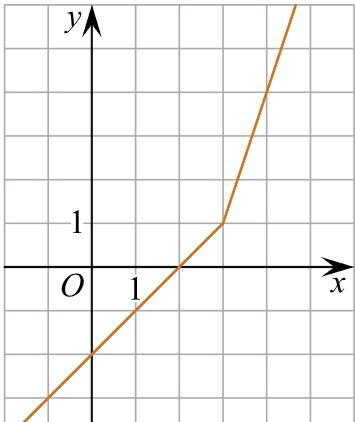
\includegraphics[align=t, width=\linewidth]{\picpath/K-L2}
		\end{minipage}
		\item Найдите точку максимума функции: \( y=x^2-48x+17 \).
		\item Найдите точку максимума функции: \( y = - \dfrac{16}{x}+x+3 \).
		\item Найдите наименьшее значение функции: \( y = (x-8)e^{x-7} \) на отрезке \( [6;8] \).
	\end{listofex}
	\newpage
	\title{Домашняя работа}
	\begin{listofex}
		\item Решите уравнения:
		\begin{tasks}(1)
			\task \( (x-6)^2=-24x \),
			\task \( \dfrac{1}{4x-1}=5 \),
			\task \( \sqrt{-72-17x}=-x \).
		\end{tasks}
		\item Найдите значение выражения:
		\begin{tasks}(2)
			\task \( \left( \mfrac{2}{4}{7} - 2,5 \right) : \dfrac{1}{70} \),
			\task \( \dfrac{1,23 \cdot 45,7}{12,3 \cdot 0,457} \).
		\end{tasks}
		%\item
		%\begin{minipage}[t]{\bodywidth}
		%	На рисунке изображён график функции вида \[ f(x)=ax+|bx+c|+d, \] где числа \(a, b, c, d\) --- целые.\\ Найдите корень уравнения \(ax+d=19\).
		%\end{minipage}
		%\hspace{0.02\linewidth}
		%\begin{minipage}[t]{\picwidth}
		%	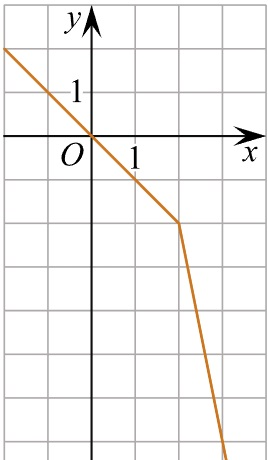
\includegraphics[align=t, width=\linewidth]{\picpath/K-L7}
		%\end{minipage}
		%4
		\item
		\begin{minipage}[t]{\bodywidth}
			На рисунке изображён график функции вида \[ f(x)=ax-|bx+c|+d, \] где числа \(a, b, c, d\) --- целые.\\ Найдите корень уравнения \(ax=d\).
		\end{minipage}
		\hspace{0.02\linewidth}
		\begin{minipage}[t]{\picwidth}
			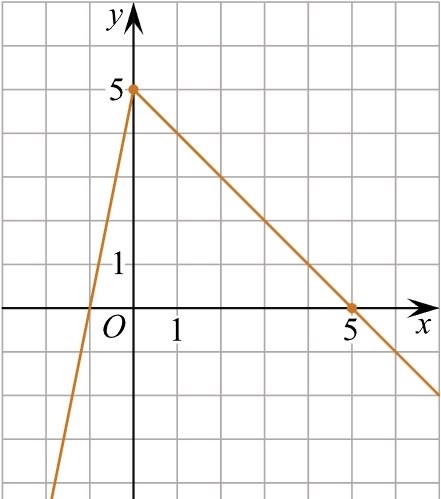
\includegraphics[align=t, width=\linewidth]{\picpath/K-L10}
		\end{minipage}
		\item Найдите точку максимума функции: \( y=x+\dfrac{9}{x} \) на отрезке \( [1;10] \).
		\item Найдите наименьшее значение функции: \( y = (x+16)e^{x-16} \) на отрезке \( [6;8] \).
	\end{listofex}
\end{consultation}
%END_FOLD